%% abtex2-modelo-projeto-pesquisa.tex, v<VERSION> laurocesar
%% Copyright 2012-2015 by abnTeX2 group at http://www.abntex.net.br/
%%
%% This work may be distributed and/or modified under the
%% conditions of the LaTeX Project Public License, either version 1.3
%% of this license or (at your option) any later version.
%% The latest version of this license is in
%% http://www.latex-project.org/lppl.txt
%% and version 1.3 or later is part of all distributions of LaTeX
%% version 2005/12/01 or later.
%%
%% This work has the LPPL maintenance status `maintained'.
%%
%% The Current Maintainer of this work is the abnTeX2 team, led
%% by Lauro César Araujo. Further information are available on
%% http://www.abntex.net.br/
%%
%% This work consists of the files abntex2-modelo-projeto-pesquisa.tex
%% and abntex2-modelo-references.bib
%%

% ------------------------------------------------------------------------
% ------------------------------------------------------------------------
% abnTeX2: Modelo de Projeto de pesquisa em conformidade com
% ABNT NBR 15287:2011 Informação e documentação - Projeto de pesquisa -
% Apresentação
% ------------------------------------------------------------------------
% ------------------------------------------------------------------------

\documentclass[
% -- opções da classe memoir --
12pt,				% tamanho da fonte
openright,			% capítulos começam em pág ímpar (insere página vazia caso preciso)
oneside,			% para impressão em recto e verso. Oposto a oneside
a4paper,			% tamanho do papel.
% -- opções da classe abntex2 --
% chapter=TITLE,		% títulos de capítulos convertidos em letras maiúsculas
% section=TITLE,		% títulos de seções convertidos em letras maiúsculas
% subsection=TITLE,	% títulos de subseções convertidos em letras maiúsculas
% subsubsection=TITLE,% títulos de subsubseções convertidos em letras maiúsculas
% -- opções do pacote babel --
english,			% idioma adicional para hifenização
brazil,				% o último idioma é o principal do documento
]{abntex2}


% ---
% PACOTES
% ---

% ---
% Pacotes fundamentais
% ---
\usepackage{lmodern}			% Usa a fonte Latin Modern
\usepackage[T1]{fontenc}		% Selecao de codigos de fonte.
\usepackage[utf8]{inputenc}		% Codificacao do documento (conversão automática dos acentos)
\usepackage{indentfirst}		% Indenta o primeiro parágrafo de cada seção.
\usepackage{color}				% Controle das cores
\usepackage{graphicx}			% Inclusão de gráficos
\usepackage{microtype} 			% para melhorias de justificação
\usepackage{amsmath,amssymb,amstext}
\usepackage{setspace}
\usepackage{float}

% ---
% Pacotes e definições adcionais, para adequações especificas
\usepackage{tikz}
\usepackage{pdflscape}			% para ambiente landscape
\usepackage{pgfgantt}			% cronograma estilo gráfico de gantt
\usetikzlibrary{backgrounds}
\definecolor{done}{RGB}{120, 180, 120}
\definecolor{do}{RGB}{180, 120, 120}

% ---

% ---
% Pacotes adicionais, usados apenas no âmbito do Modelo Canônico do abnteX2
% ---
\usepackage{lipsum}				% para geração de dummy text
% ---

% JSON
\usepackage{listings}
% 2 columns
\usepackage{parcolumns}
\usepackage{adjustbox}

% Image
\usepackage{wrapfig}

% ---
% Pacotes de citações
% ---
\usepackage[brazilian,hyperpageref]{backref}            % Paginas com as citações
\usepackage[alf]{abntex2cite}				% Citações padrão ABNT
% \usepackage{abntex2cite}

% ---
% CONFIGURAÇÕES DE PACOTES
% ---

% ---
% Configurações do pacote backref
% Usado sem a opção hyperpageref de backref
\renewcommand{\backrefpagesname}{Citado na(s) página(s):~}
% Texto padrão antes do número das páginas
\renewcommand{\backref}{}
% Define os textos da citação
\renewcommand*{\backrefalt}[4]{
  \ifcase #1 %
  Nenhuma citação no texto.%
  \or
  Citado na página #2.%
  \else
  Citado #1 vezes nas páginas #2.%
  \fi}%
% ---

% ---
% Informações de dados para CAPA e FOLHA DE ROSTO
% ---
\titulo{Avaliação do impacto dos jogadores em modelos preditivos no jogo Dota2}
\vspace{2cm}
\autor{Andryas Waurzenczak}
\local{Curitiba}
\data{2019}
\instituicao{Universidade Federal do Paraná
  \par
  Setor de Ciências Exatas
  \par
  Departamento de Estatística
}
\orientador[Orientador:]{Prof. Dr. Walmes Marques Zeviani}
\tipotrabalho{Projeto de Pesquisa}
% O preambulo deve conter o tipo do trabalho, o objetivo,
% o nome da instituição e a área de concentração
\preambulo{Projeto de Pesquisa apresentado à disciplina Laboratório A
  do Curso de Graduação em Estatística da Universidade Federal do Paraná,
  como requisito para elaboração do Trabalho de Conclusão de Curso}
% ---

% ---
% Configurações de aparência do PDF final

% alterando o aspecto da cor azul
\definecolor{blue}{RGB}{41,5,195}

% informações do PDF
\makeatletter
\hypersetup{
  % pagebackref=true,
  pdftitle={\@title},
  pdfauthor={\@author},
  pdfsubject={\imprimirpreambulo},
  pdfcreator={LaTeX with abnTeX2},
  pdfkeywords={abnt}{latex}{abntex}{abntex2}{projeto de pesquisa},
  colorlinks=true,	% false: boxed links; true: colored links
  linkcolor=blue,     % color of internal links
  citecolor=blue, % color of links to bibliography
  filecolor=magenta, % color of file links
  urlcolor=blue,
  bookmarksdepth=4
}
\addto\captionsbrazil{
  \renewcommand{\bibname}{REFER\^ENCIAS}
}
\makeatother
% ---

% ---
% Espaçamentos entre linhas e parágrafos
% ---

% O tamanho do parágrafo é dado por:
\setlength{\parindent}{1.3cm}

% Controle do espaçamento entre um parágrafo e outro:
\setlength{\parskip}{0.2cm}  % tente também \onelineskip


% ---
% compila o indice
% ---
\makeindex
% ---

% ----
% Início do documento
% ----
\begin{document}

% Seleciona o idioma do documento (conforme pacotes do babel)
% \selectlanguage{english}
\selectlanguage{brazil}

% Retira espaço extra obsoleto entre as frases.
% \frenchspacing

% ----------------------------------------------------------
% ELEMENTOS PRÉ-TEXTUAIS
% ----------------------------------------------------------
% \pretextual

% ---
% Capa
% ---
\tikz[remember picture,overlay] \node[opacity=0.9,inner sep=0pt] at
(current page.center){
  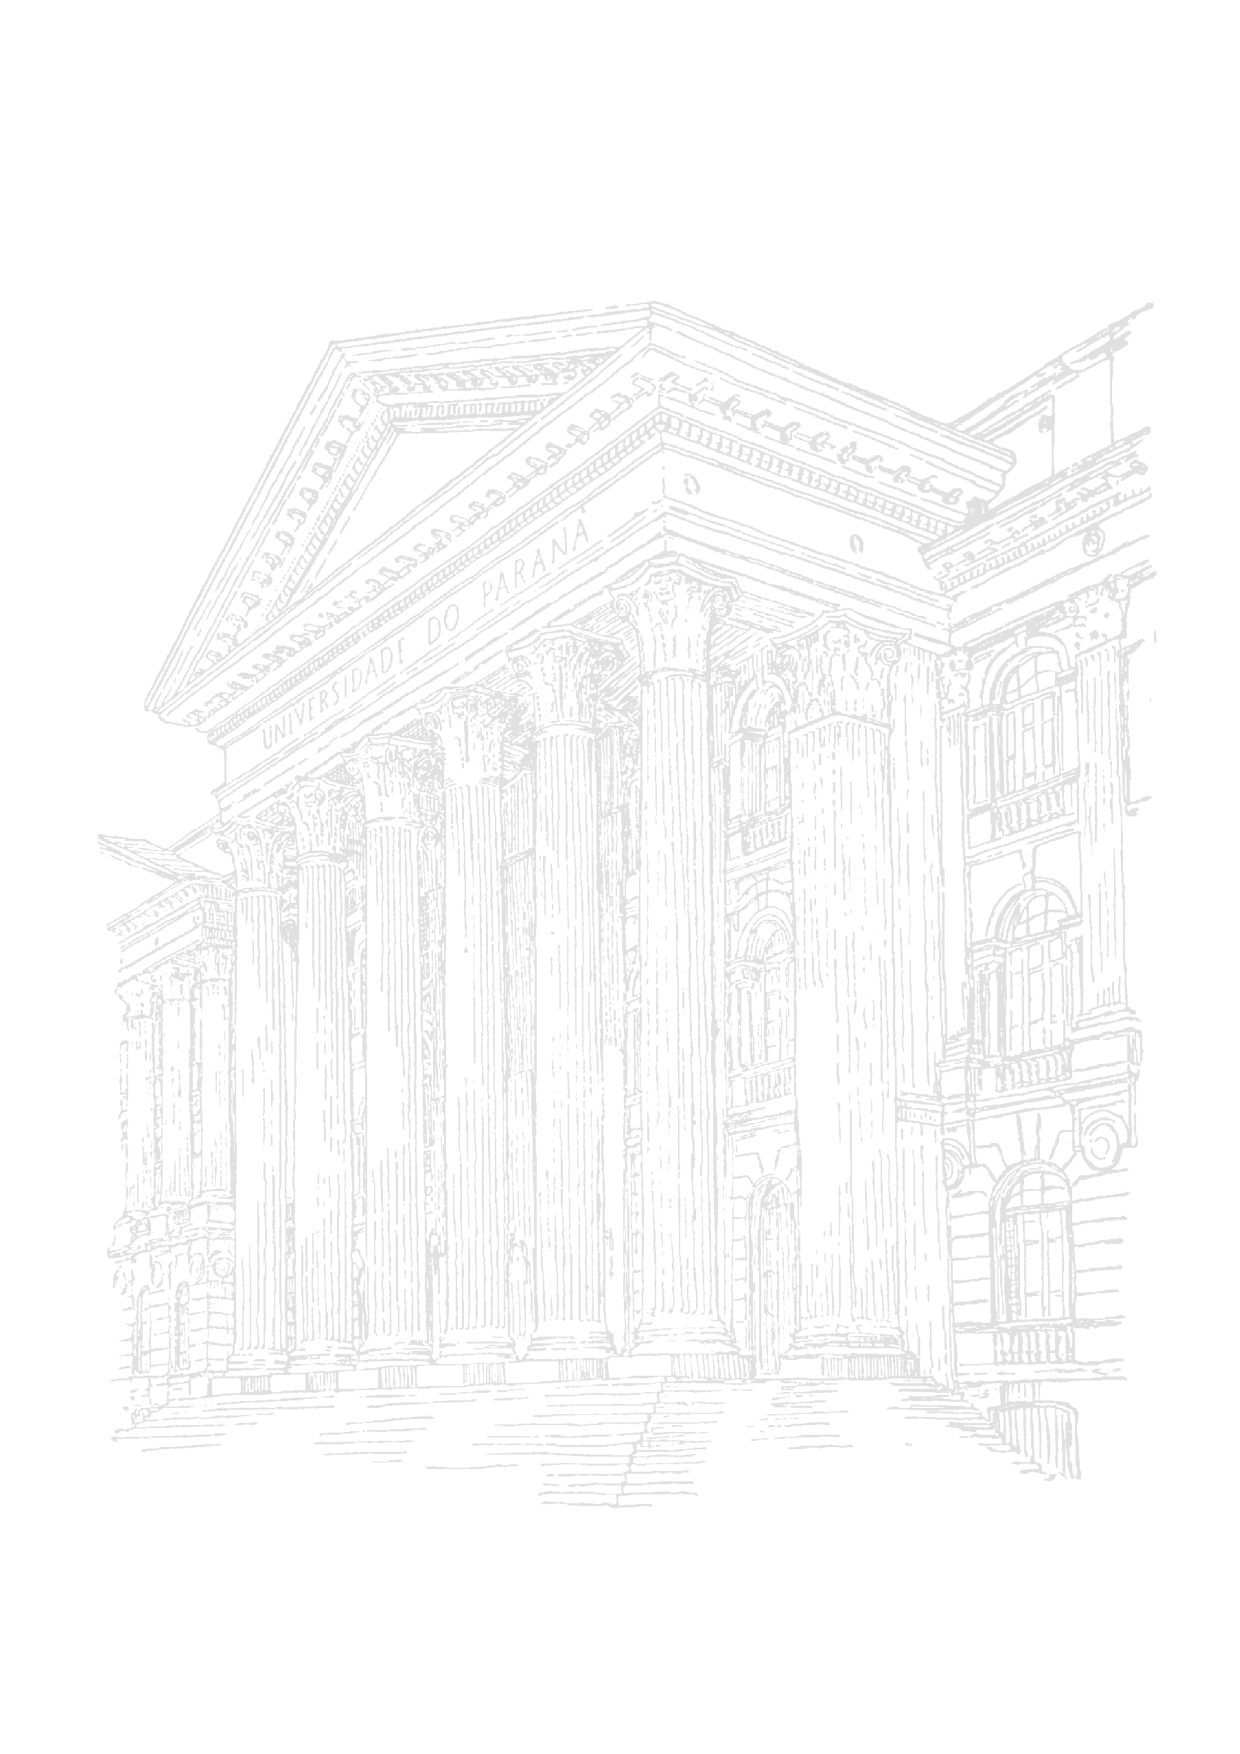
\includegraphics[width=\paperwidth,
  height=\paperheight]{image/ufpr_bg}};

\begin{center}
  {\Large \textsf{Universidade Federal do Paraná}} \\
\end{center}
\imprimircapa

% ---

% ---
% Folha de rosto
% ---
\imprimirfolhaderosto
% ---

% ---
% inserir o sumario
% ---
\pdfbookmark[0]{\contentsname}{toc}
\tableofcontents*
\cleardoublepage
% ---


% ----------------------------------------------------------
% ELEMENTOS TEXTUAIS
% ----------------------------------------------------------
\textual

% ----------------------------------------------------------
% Introdução
% ----------------------------------------------------------
\chapter{Introdução}
\label{cha:introducao}


Dos astrágalos da antiga Grécia aos jogos de console e computador do século XXI.
Ao longo da trágetoria humana os jogos tem desempenhado um papel essêncial para
o desenvolvimento da ciência e da tecnologia. Atualmente os jogos tem servido
como verdadeiros laborátorios para o desenvolvimento de áreas como Machine
Learning e Inteligencia Artificial, isto por que tem-se, geralmente, uma grande
quantidade de dados disponiveis e ambientes controlados. \cite{silva2017moba}

Um dos jogos que tem chamado a atenção de pesquisadores e, também, de
grandes empresários é o jogo Dota2\footnote{http://dota2.com/}. Diversos
trabalhos relacionados ao jogo foram feitos, como por exemplo, a instituição sem
fins lucrativos OpenAI\footnote{https://www.openai.com/}, financiada por um dos
grandes visionários do mundo atualmente,  Elon
Musk\footnote{https://en.wikipedia.org/wiki/Elon\_Musk}, que criou o primeiro programa capaz de
``jogar o jogo'' e que teve seu poder computacional demonstrado no The International de 2017 e 2018.
Além de vários outros trabalhos que visavam, não somente a criação de algoritmos capazes de jogar o
jogo mas também, prever o desfecho da partida.

O jogo é atraente tanto visualmente como estratégicamente, baseado em jogos de Real-time Strategy
(RTS),  o jogo acontece em uma arena fechada que é divida em dois times de cinco jogadores, os
Iluminados (The Radiant) e os Temidos (The Dire). O objetivo central do jogo é destruir o Ancestral
do time adversário, que fica localizado no centro de cada base. Para tal, é necessário passar por
diversas etapas do jogo que em sua essência são comuns a jogos de role-playing game, os famosos
RPG. Essas etapas podem ser resumidas em duas principais, à \textit{obteção de experiência}, para
que o personagem escolhido pelo jogador possa ganhar níveis e assim ficar mais forte na partida, e a
\textit{obtenção de ouro}, para poder comprar itens que aumentam os status do personagem ou dão
habilidades extras. Esses personagens escolhidos pelos jogadores são chamados de heróis, alguns são
personificações de mitologias soltas pelo mundo, como por exemplo Zeus. Cada herói possui, de forma
genérica, 5 atributos, que são: força, inteligência, agilidade, resistência a mágia e armadura.
Alguns atributos, como se pode imaginar, são mais abundânntes em uns heróis que outros, dando
diversidade ao jogo. Além disso cada herói possui caracteristicas únicas que podem se tornar tanto
uma fraqueza como uma força dependendo dos heróis escolhidos pelo time adversário. Também existe a
relação entre os herói que podem produzir combinações mais poderosas ou mais vuneráveis. Abaixo
tem-se uma imagem do mapa do jogo.


\begin{wrapfigure}{l}{0.55\textwidth}
  \begin{center}
    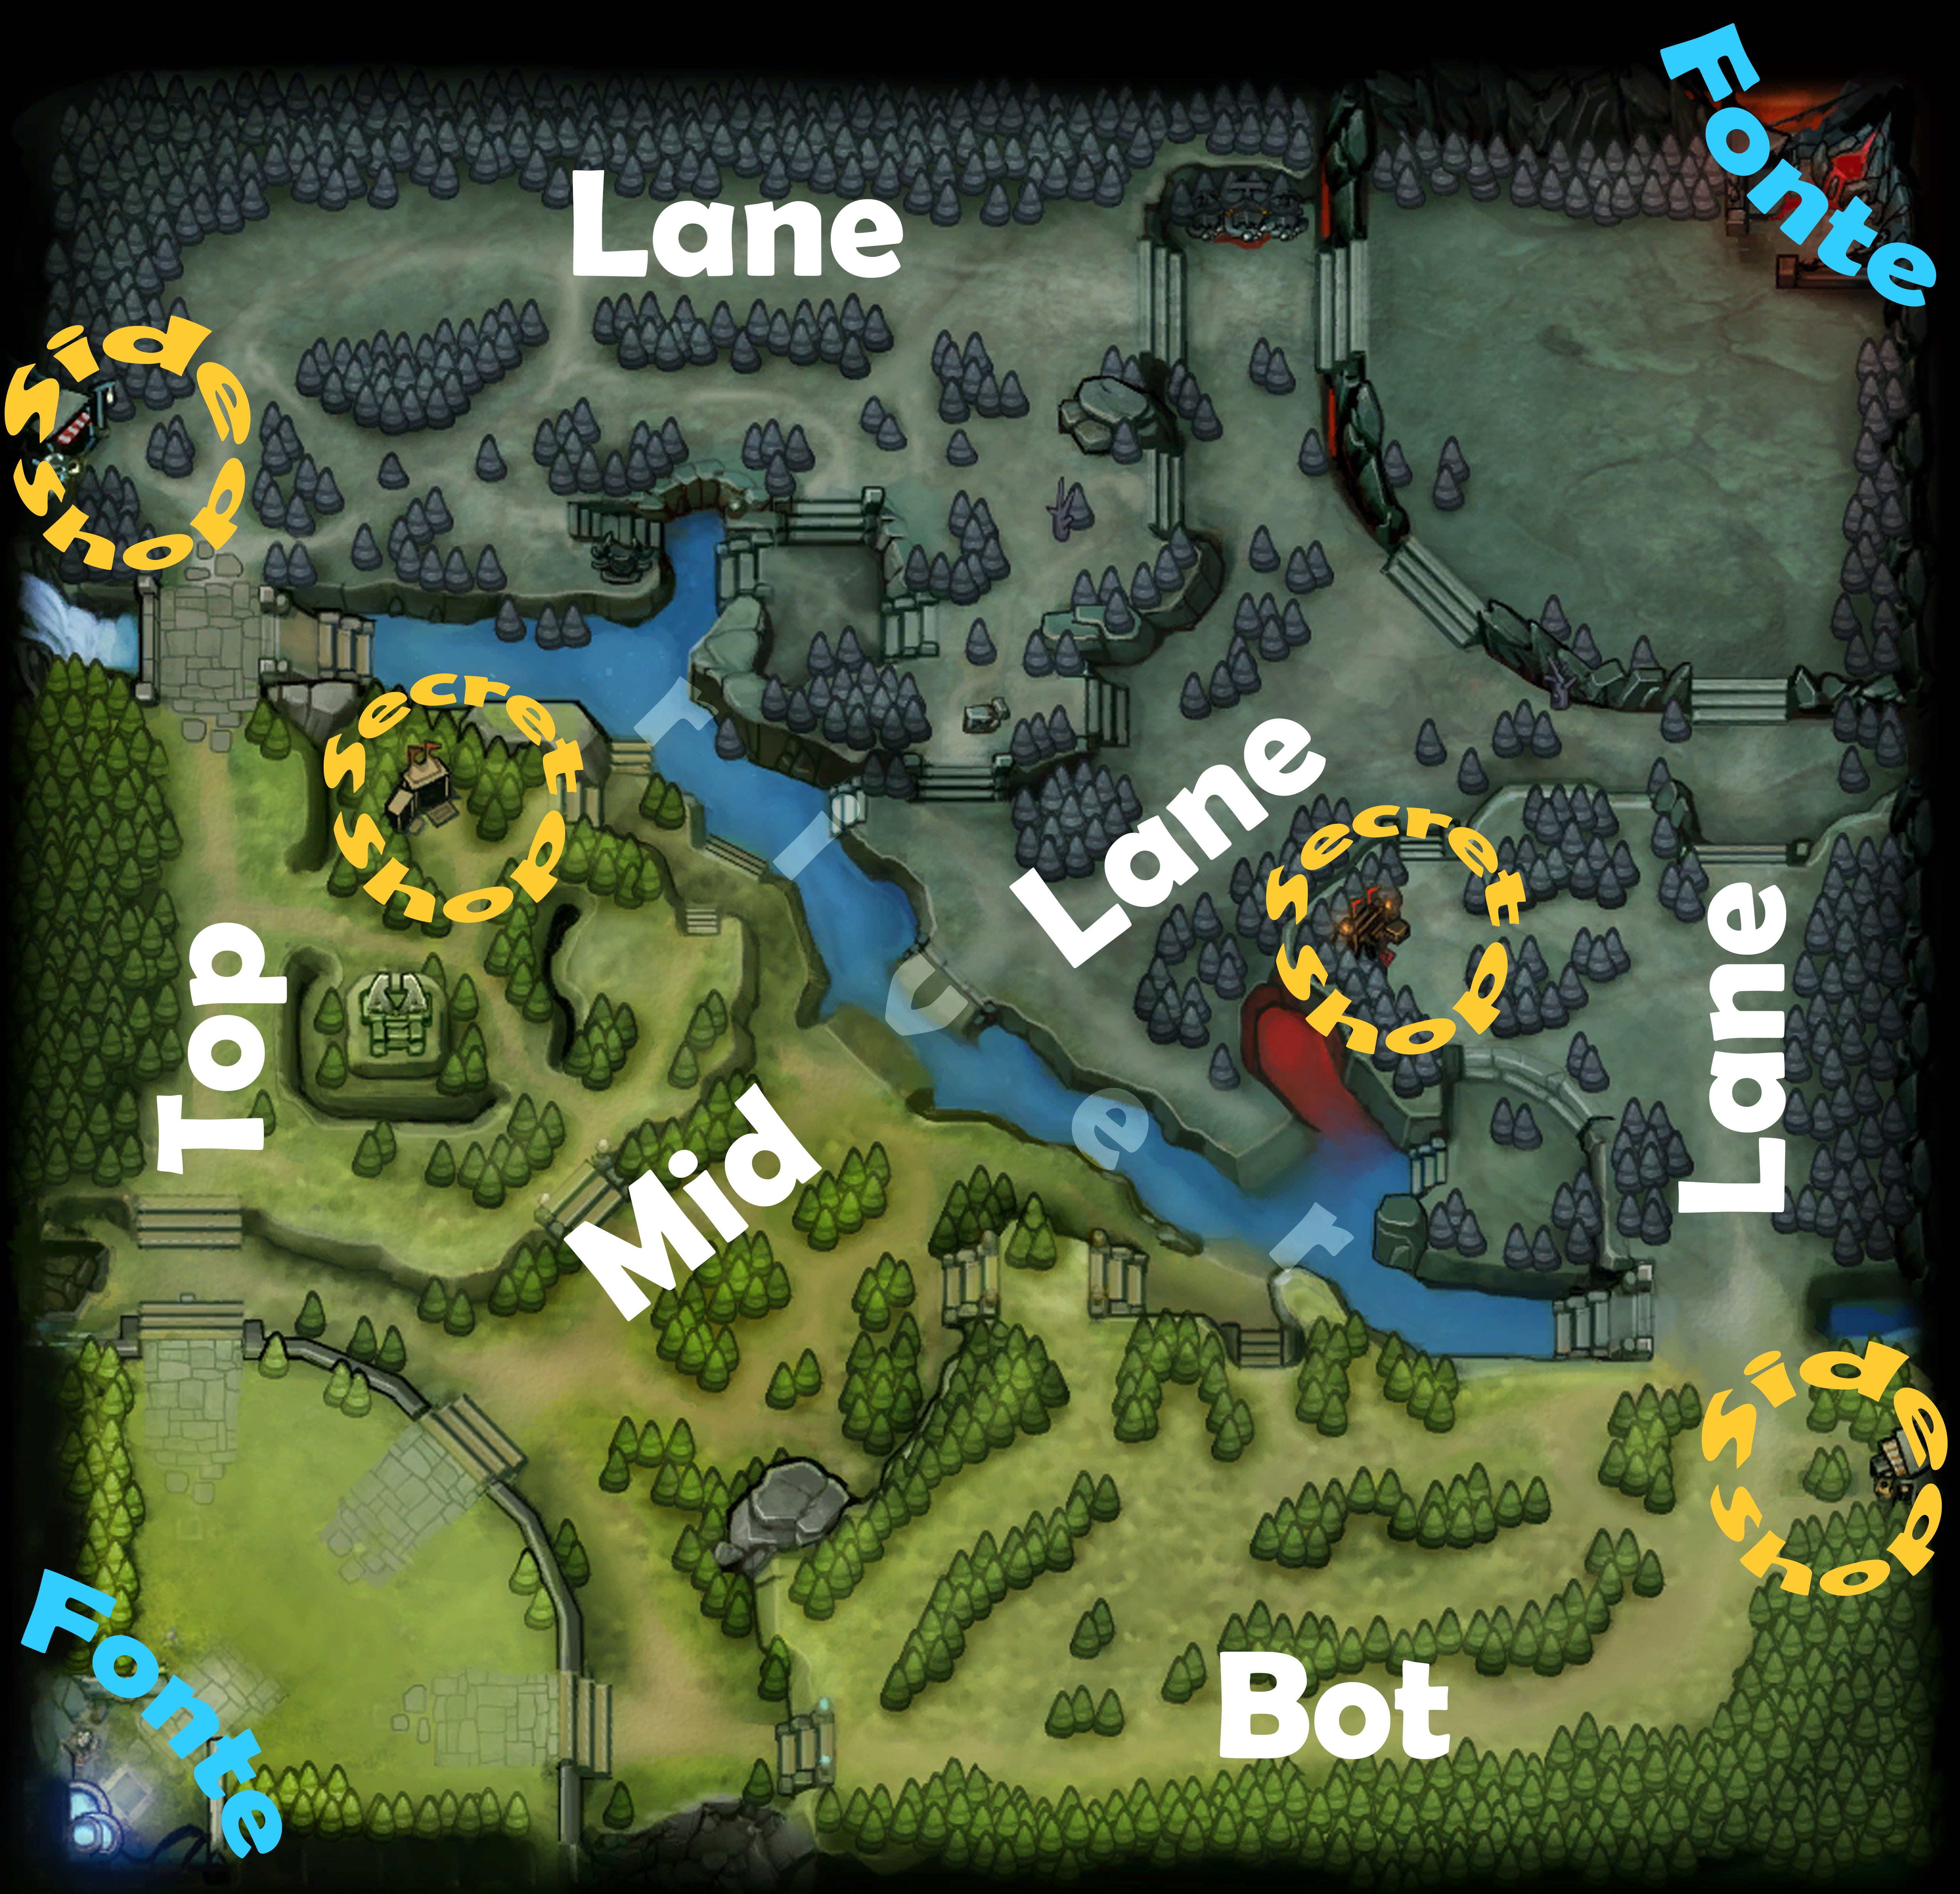
\includegraphics[width=0.48\textwidth]{image/mapa.jpeg}
    \caption{Mapa do jogo}
  \end{center}
\end{wrapfigure}

No canto inferior esquerdo tem-se então o time dos Iluminados e no canto superior direito tem-se o
time dos Temidos. Existem ao todo três caminhos, comumente chamados de mid, top e bot. Cada caminho
possui três torres de defesa, sendo que é necessário destruir sequenciamente cada torre para poder
avançar para a próxima. Nesses caminhos criaturas conhecidas como creeps surgir periodicamente e vão
avançando até o encontro com as criaturas do time adversário. Esses creeps, quando finalizados por
herói geram ouro e quando mortos próximos deles geram experiência.


Atráves de toda essa gama de opções é que o Dota2 tem conquistado seu espaço e se tornado o jogo
mais bem pago dentre os demais jogos do gênero. Abaixo tem-se em doláres a premiação total dos
últimos eventos do The International.

\begin{figure}[H]
  \begin{center}
    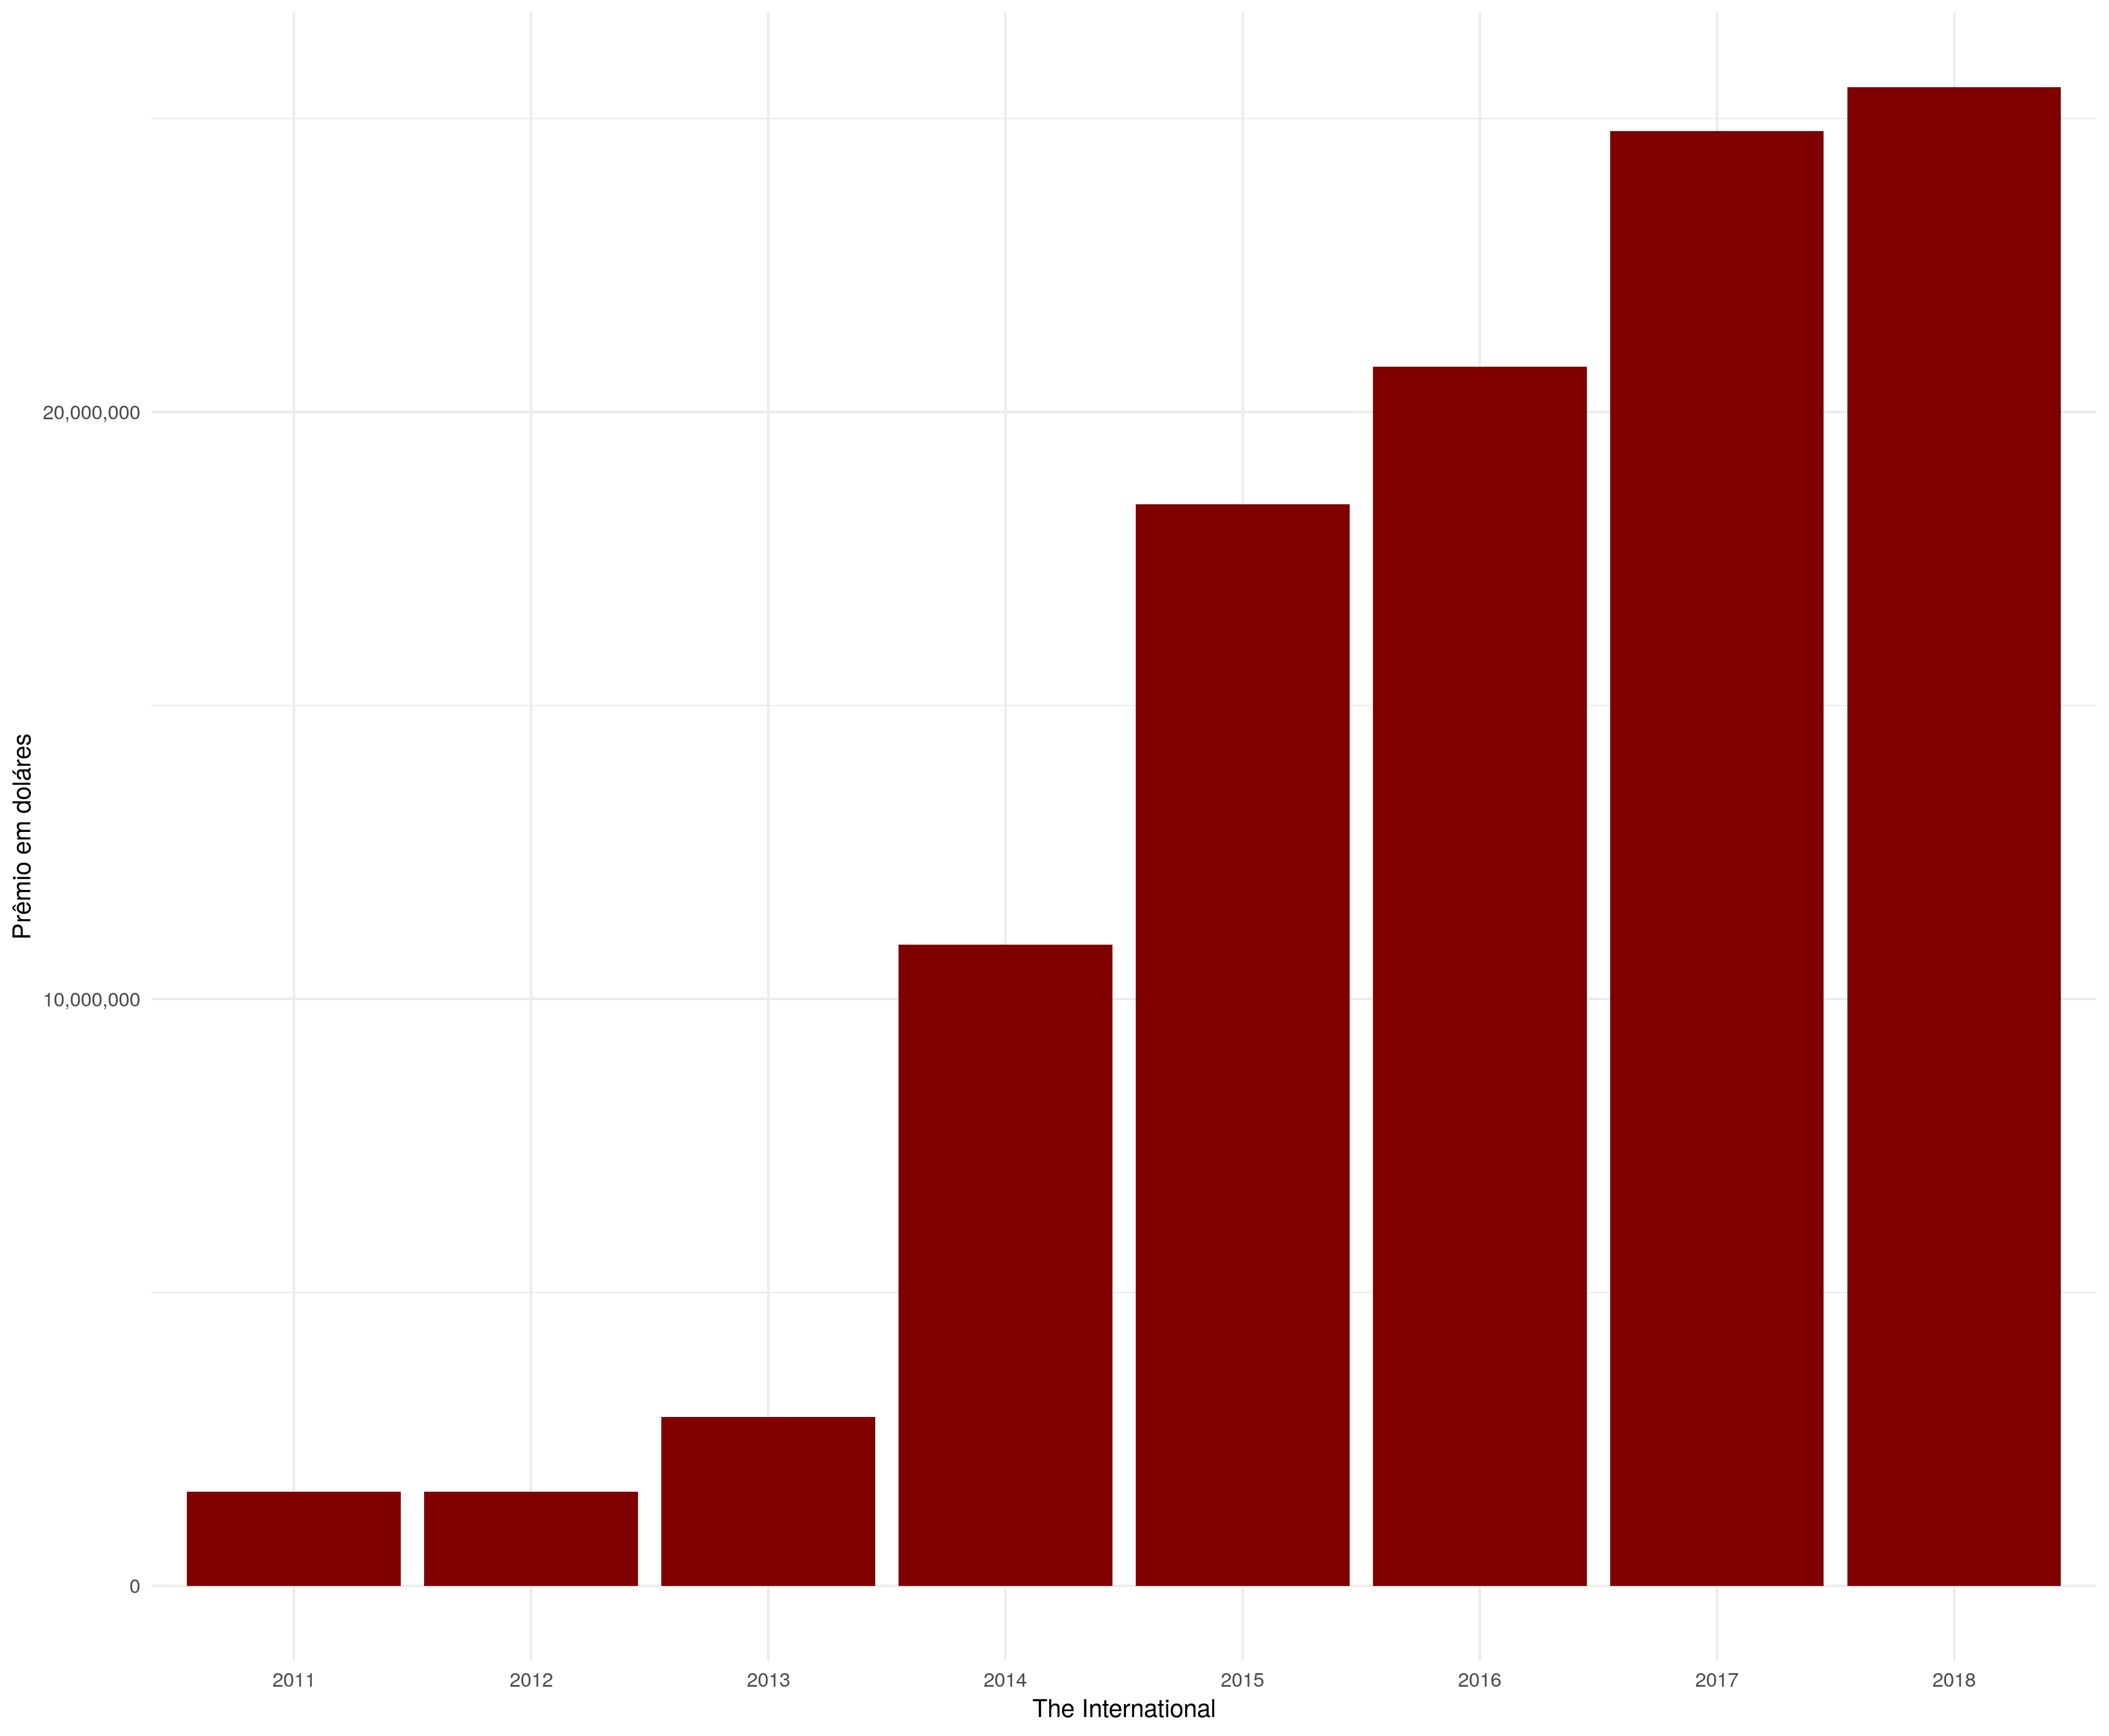
\includegraphics[width=14cm,height=10cm]{image/dotaprize.png}
    \caption{Premiação do evento principal, The International.}
  \end{center}
\end{figure}





% sendo que o objetivo principal do jogo é
% destruir a o ancestral do time adversário.
%
% Nesse sentido de prever, o presente trabalho terá como objetivo contribuir para o aprimoramento de
% modelos preditivos do jogo Dota2 incrementando covariáveis a modelos já existentes. Com o
% crescimento do mercado de online de apostas e o próprio ramo profissonal do jogo, a avaliação de
% melhores decisões no jogo se faz necessário. A maioria dos trabalhos publicados sobre o jogo que
% fazem predição, em geral, utilizam apenas informações


% Um dos esportes eletrônicos que mais tem movimentado o mercado de jogos, tanto
% Um dos jogos que mais está em alta, tanto economicamente quanto em atenção, é o jogo
% Dota2\footnote{}. Este jogo, que é o tema do trabalho, tem
% se destacado nos últimos anos principalmente por causa do seu evento principal,
% que acontece uma vez ao ano, conhecido como The International e , também, por
% ter chamado a atenção de um dos maiores empreendedores e visionários do mundo,
% Elon Musk\footnote{https://en.wikipedia.org/wiki/Elon\_Musk}, que em outubro de
% 2015 junto com mais alguns investidores emprenderam mais de 1 bilhão de doláres
% em uma instituição sem fins lucrativos conhecida como
% OpenAI\footnote{https://www.openai.com/} que em seus projetos iniciais teve como
% foco o desenvolvimento de uma inteligencia capaz de ``jogar'' o jogo
% Dota2\footnote{https://blog.openai.com/dota-2/}.


% Dota2 é um jogo eletrônico desenvolvido pela empresa
% Valve\footnote{https://www.valvesoftware.com/pt-br/} e que pode ser baixado e
% jogado gratuitamente pela plataforma de jogos
% Steam\footnote{https://steamcommunity.com/}.



% Neste evento diversas equipes profissionais se enfrentam, algumas sendo financiadas
% por grandes empresas outras por si mesmas, que atráves de treinos intensos se
% preparam para participar de diversos torneios e que atráves deles vão
% conquistando torcedores e atraindo mais audiência ao jogo.
%
% Para poder participar desse evento as
% equipes devem ficar bem colocadas em torneios menores, chamados de Majors, que
% acontecem ao redor do mundo.




% Uma das primerias teorias sobre a lei das probabilidade, que é um dos alicerces
% da ciência estatística, em suas primeiras formulações por Girolamo Cardano, teve
% como motivação, segundo \cite{bernstein1997desafio}, o desenvolvimento de uma
% teoria dos jogos, e não uma teoria de probabilidades.

% Ainda no século XXI os jogos continuam a fomentar o desenvolvimento de novas
% tecnologias, hoje ouvesse muito sobre Inteligência Artificial (AI) e Máquina de
% Aprendizado (ML) que são ramificações da estatística que ganharam vida
% própria. No entanto, o progresso e o sucesso dessas áreas está ligada, de certa
% forma, aos jogos, pois se no momento em que se consegue fazer um computador
% jogar um jogo tão complexo como Dota2, por exemplo, onde deve-se tomar diversar
% decisões simultãneas instante à instante, qual seria a dificuldade de
% externelizar esse conhecimento para o mundo real? Pode-se dizer que jogos de
% computadores são verdadeiros laborátorios para o desenvolvimento e o progresso da
% ciência como um todo \cite{silva2017moba}.
%
% Não obstante, os jogos movimentam a economia, fatos sobre isso podem ser
% observados em estatísticas que revistas especializadas sobre mercados de jogos
% disponibilizam, segundo a \cite{newzoo2018global}, por exemplo, o mercado de
% jogos no ano de 2018 teve um lucro de aproximadamente de 134.9 bilhões de
% doláres, onde 63.2 bilhões para jogos de mobile, 38.3 bilhões para jogos de
% console e 33.4 bilhões para jogos de computador. E além disso abriu espaço
% para diversos sistemas de apostas que fornecem serviços nos mais
% variados jogos eletrônicos, alguns exemplos são
% gg.bet\footnote{https://gg.bet/pt/betting},
% pinnacle\footnote{https://www.pinnacle.com/pt/}.
%
% Este trabalho tem como objetivo contribuir com a ciência dos esportes
% eletrônicos, no genêro MOBA (Multiplayer Online Battle Arena) no jogo
% DotA2\footnote{www.dota2.com}. A escolha desse jogo se deve a alguns fatores,
% primeiramente pela preferência do autor, segundo por ser o eSport mais bem pago
% de todos os tempos e por último porque Elon Musk, um dos maiores empreendedores
% e visionarios do mundo, investiu em um projeto conhecido como
% openAI\footnote{https://openai.com/} que desenvolveu algoritmos inteligentes
% capazes de jogar o jogo pela primeira vez no The International de 2017 o que
% chocou a comunidade e fez o jogo ganhar mais espaço e atrair mais cientistas das
% mais diversas áreas.


% ----------------------------------------------------------
% Objetivos
% ----------------------------------------------------------
\chapter{Objetivos}
% \label{cha:objetivos}

\section{Objetivos Gerais}
% \label{sec:objetivosgerais}

Avaliar se inclusão de variáveis relacionadas ao jogador tem impacto
significativo em prever o desfecho da partida após a seleção dos heróis no
jogo Dota2.

\section{Objetivos Específicos}
% \label{sec:objetivosespecificos}

\begin{itemize}
\item Apresentar a temática eSports

\item Apresentar a forma de coleta dos dados via API

\item Apresentar e Implementar o processo de tabulação dos dados para fins de
modelagem

\item Ajustar, validar e comparar diferentes modelos com e sem a informação dos
jogadores, atráves de métricas de desempenho

\end{itemize}

% ----------------------------------------------------------
  % Materiais e Métodos
% ----------------------------------------------------------
\chapter{Materiais e Métodos}
\label{cha:materiaisemetodos}

\section{Materiais}
\label{sec:materiais}

\subsection{Sobre os Dados}

Os dados são coletados atráves de uma \emph{Application programming interface}
(API) da plataforma de jogos Steam\footnote{https://store.steampowered.com/about/}.
Este serviço é disponivel somente para usúarios que tenham comprado algum jogo
da plataforma, pois, somente após a compra é disponibilizado uma chave de
acesso. Cada chave pode fazer uma quantidade limitada de requisições em um curto
espaço de tempo, para este trabalho cujo o objetivo é avaliar variáveis
relacionadas ao jogador presente em cada partida tem-se um primeiro problema na
aquisição dos dados, sendo que para cada partida coletada é necessário buscar o
histórico de cada jogador presente na partida, isto faz com que a quantidade de
requisições cresca tendo assim problemas na coleta dos dados. Na seção \ref{sec:coletadosdados}
 é apresentado o fluxo de execução programada e dado
maiores detalhes para contornar este problema.

\subsection{Recursos Computacionais}

Para as análises e desenvolvimento do trabalho será utilizado o software R \cite{rcoreteam}.
Para o armazenamento e a tabulação das informações será
utilizado dois banco de dados, o primeiro é o
MongoDB\footnote{https://www.mongodb.com/}, que é um banco de dados
destruturados e o segundo é o MySQL\footnote{https://www.mysql.com/} que é
um banco de dados relacional para a tabulação dos dados.


\subsection{Coleta dos Dados}
\label{sec:coletadosdados}

O processo de coleta dos dados é feito atráves de programas em R que ficam
coletando dados 24 horas por dias fazendo requisições na API da plataforma
Steam para a aquisião de novos IDs de partidas, preparando as informações da
partida e dos jogadores que estão presentes nela e armazenando no banco de dados
MongoDB.


O fluxo abaixo trás mais detalhes deste processo. As caixas em cinzas é a ordem
da execução/fase de cada programa.

\begin{figure}[H]
  \begin{center}
    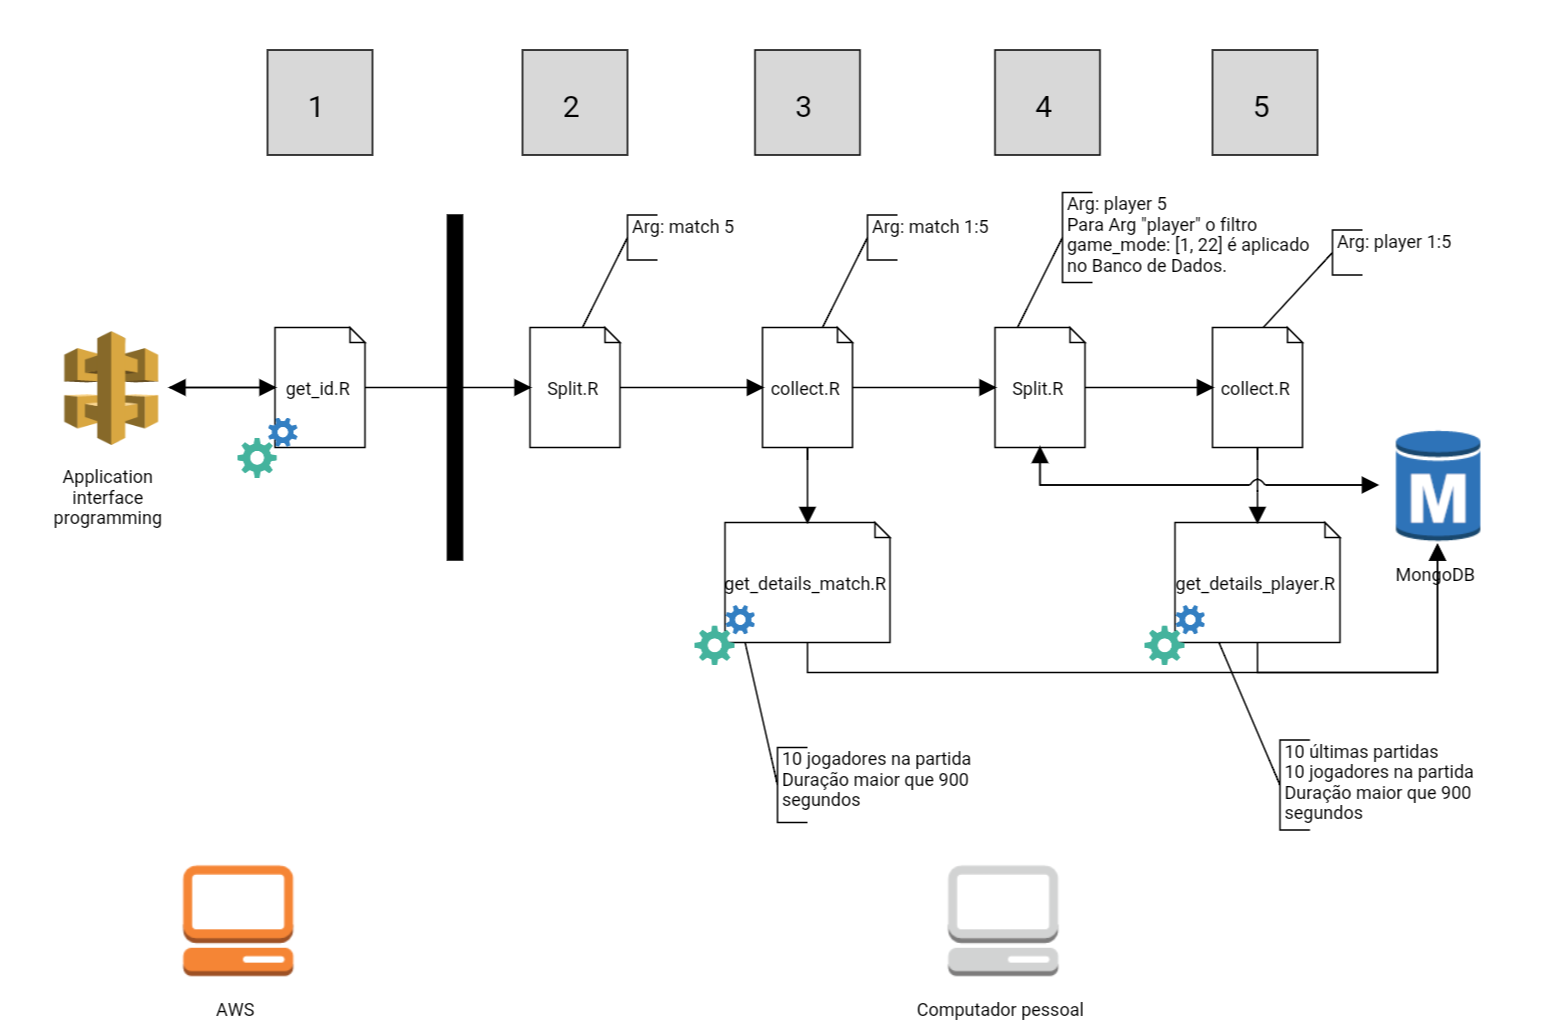
\includegraphics[width=14cm,height=10cm]{image/collect.png}
    \caption{Fluxo do processo de coleta dos dados}
  \end{center}
\end{figure}

\begin{enumerate}
\item O programa \textbf{get\_id.R} faz uma requisição na API e retorna com as
  partidas que estão acontencendo no momento da requisição, os IDs dessas
  partidas são processados e armazenados, e repete-se o processo de tempos em
  tempos (120 segundos). É necessário o armazenamento dos IDs para uma coleta
  posterior das informações da partida após seu termino, pois é possível
  coletar as informações da partida se estas ainda não terminaram. Deve-se
  deixa-lo rodando em uma máquina 24 horas por dia com conexão estável com a
  internet. Para este trabalho um computador da
  Amazon\footnote{https://aws.amazon.com/pt/} está sendo utilizado.

\item O programa \textbf{split.R} divide o arquivo  gerado pelo programa
  \textbf{get\_id.R}, que é um vetor com \textbf{n} IDs coletados que são
  separados em \textbf{j} partes, para cada parte uma chave de acesso é
  necessária, para processar mais rapidamente as informaçõesda partida.

\item O programa \textbf{collect.R} lê cada um dos arquivos gerados pelo
  programa \textbf{split.R} e cria uma instância do R, para cada um, que irá
  coletas as informações da partida e armazena-las no MongoDB.

\item Após coletar as informações da partida o arquivo \textbf{split.R}
  conecta-se ao banco de dados, seleciona todas as partidas coletadas e pega os
  IDs de todos os jogadores que compoem a partida. Após isso divide em
  \textbf{j} arquivos .RData, cada qual com informações do ID da partida e o ID
  do jogador que fez parte dela.

\item Por último o programa \textbf{collect.R} processa cada arquivo com o ID da
  partida e o ID do jogador varrendo o histórico do jogador coletando as suas
  últimas 10 partidas e armazenando-as no banco de dados MongoDB.

\end{enumerate}

Como exemplo, tem-se abaixo as informações de uma única partida coletada. O
campo \emph{players} está oculto na primeira representação pois este campo
contém as informações de cada jogador na partida, e é demasiadamente longo.
Para ilustrar foi selecionado apenas o primeiro jogador que está na próxima
página.


\lstset{
  % basicstyle=\tiny
  string=[s]{"}{"},
  stringstyle=\color{blue},
  comment=[l]{:},
  commentstyle=\color{black},
  basicstyle=\tiny
}

\begin{center}
\begin{minipage}{.5\textwidth}
\begin{lstlisting}[caption=match]{Name}
[
  {
    "players": ...,
    "radiant_win": false,
    "duration": 1869,
    "pre_game_duration": 90,
    "start_time": 1549408252,
    "match_id": 4394571998,
    "match_seq_num": 3799941136,
    "tower_status_radiant": 390,
    "tower_status_dire": 1974,
    "barracks_status_radiant": 51,
    "barracks_status_dire": 63,
    "cluster": 184,
    "first_blood_time": 97,
    "lobby_type": 7,
    "human_players": 10,
    "leagueid": 0,
    "positive_votes": 0,
    "negative_votes": 0,
    "game_mode": 22,
    "flags": 1,
    "engine": 1,
    "radiant_score": 19,
    "dire_score": 36,
    "picks_bans": [
      {
        "is_pick": false,
        "hero_id": 8,
        "team": 0,
        "order": 0
      },
      {
        "is_pick": false,
        "hero_id": 44,
        "team": 0,
        "order": 1
      }
    ]
  }
]
\end{lstlisting}
\end{minipage}
\end{center}

\begin{adjustbox}{width=1.3\textwidth, height=12cm, keepaspectratio}
\begin{minipage}{.6\textwidth}
\begin{lstlisting}[caption="players", captionpos=b]{Name}
  [{
    "players": [
    {
      "account_id": 292190898,
      "player_slot": 0,
      "hero_id": 54,
      "item_0": 50,
      "item_1": 151,
      "item_2": 11,
      "item_3": 252,
      "item_4": 112,
      "item_5": 36,
      "backpack_0": 0,
      "backpack_1": 0,
      "backpack_2": 0,
      "kills": 2,
      "deaths": 5,
      "assists": 6,
      "leaver_status": 0,
      "last_hits": 201,
      "denies": 28,
      "gold_per_min": 440,
      "xp_per_min": 462,
      "level": 18,
      "hero_damage": 16096,
      "tower_damage": 2198,
      "hero_healing": 1040,
      "gold": 524,
      "gold_spent": 13110,
      "scaled_hero_damage": 9318,
      "scaled_tower_damage": 1216,
      "scaled_hero_healing": 603,
      "ability_upgrades":
      {
        "ability": 5250,
        "time": 284,
        "level": 1
      },
      {
        "ability": 5251,
        "time": 395,
        "level": 2
      },
      {
        "ability": 5250,
        "time": 490,
        "level": 3
      },
      {
        "ability": 5249,
        "time": 566,
        "level": 4
      },
      {
        "ability": 5250,
        "time": 688,
        "level": 5
      },
      ...
    },
    ...
    ]
\end{lstlisting}
\end{minipage}\hfill
\begin{minipage}{.6\textwidth}
\begin{lstlisting}[caption="players.ability\_upgrades", captionpos=b]{Name}
  [{
    ...,
    {
      "ability": 5252,
      "time": 769,
      "level": 6
    },
    {
      "ability": 5249,
      "time": 846,
      "level": 7
    },
    {
      "ability": 5250,
      "time": 975,
      "level": 8
    },
    {
      "ability": 5251,
      "time": 1067,
      "level": 9
    },
    {
      "ability": 5906,
      "time": 1158,
      "level": 10
    },
    {
      "ability": 5249,
      "time": 1202,
      "level": 11
    },
    {
      "ability": 5253,
      "time": 1333,
      "level": 12
    },
    {
      "ability": 5249,
      "time": 1438,
      "level": 13
    },
    {
      "ability": 5251,
      "time": 1515,
      "level": 14
    },
    {
      "ability": 5939,
      "time": 1718,
      "level": 15
    },
    {
      "ability": 5251,
      "time": 1860,
      "level": 16
    },
    {
      "ability": 5252,
      "time": 2169,
      "level": 17
    }
    ]
  }
\end{lstlisting}
\end{minipage}
\end{adjustbox}

\section{Métodos}
\label{sec:metodos}

Neste trabalho será utilizado tanto modelos estatísticos, como por exemplo o
modelo logistico, quanto algoritmo de machine learning e será escolhido o melhor
dentre eles. Também se fará uso de técnicas de treinamento e o uso de métricas
para avaliar o desempenho dos modelos, como por exemplo validação cruzada, para
o treinamento, e a curva ROC para escolha de um ponto de corte.

% Predizer partidas de jogos MOBA, em especifico Dota2, podem ter duas abordagens: antes do inicio do
% jogo e durante. A primeira pode-se feita em dois instantes antes da escolha dos herois e depois da
% escolha dos herois. Antes da escolha dos herois as informações disponiveis serão somente o historico
% dos jogadores. Nessa abordagem o poder preditivo tem um desempenho um pouco
% melhor que jogar uma moeda, como o blabla mostrou em seu trabalho com times profissionais, no
% entanto para questões de apostas pode ser o caminho mais interessante sendo que nesse tipo de
% aposta, onde não se tem a informação dos personagens, o ganho é maior de forma geral. Contudo existe
% também formas de apostar após a escolha dos heróis 



% ----------------------------------------------------------
 % Cronograma
% ----------------------------------------------------------
\begin{landscape}
  \chapter{Cronograma de Atividades}
  \label{cha:cronograma}

% \vspace{-0.2cm}
\begin{center}
\begin{SingleSpacing}
\hspace{-1.5cm}
% \resizebox{1\textwidth}{0.7\textheight}{
  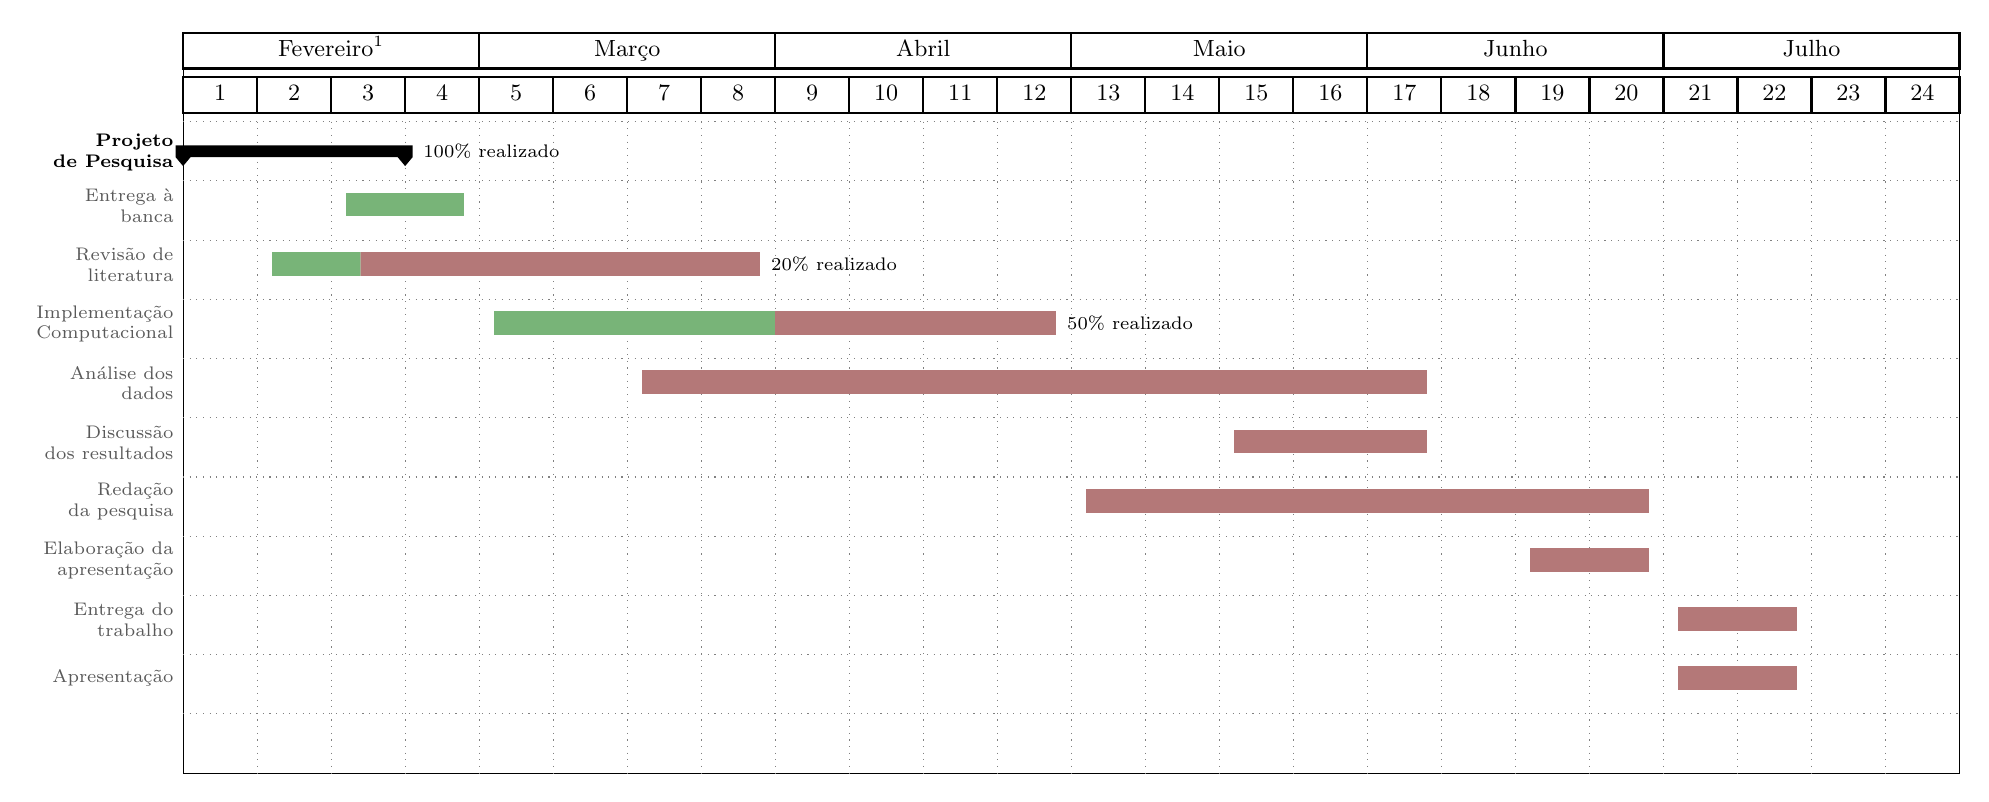
\begin{tikzpicture}[thick, scale=0.94, every node/.style={scale=0.94}]
  \begin{ganttchart}[
    canvas/.append style={fill=none},
    y unit title=0.6cm, % Size da indicação do tempo
    y unit chart=0.8cm, % Size do altura das colunas
    x unit= 10mm, % largura das celulas
    vgrid={*1{black!50, dotted}}, % grid cinza vertical
    hgrid={*1{black!50, dotted}}, % grid cinza horizontal
    title height=0.8, % Size dos dias
    bar/.style={fill=done},
    bar incomplete/.append style={fill=do},
    bar label node/.append style={align=right},
    bar label font=\scriptsize\color{black!65},
    group label font=\bfseries\scriptsize\color{black},
    group left peak width=0.2,
    group right peak width=0.2,
    group left peak height=0.15,
    group right peak height=0.15,
    bar height=0.6, % size das barras de tarefas
    bar left shift=.2, bar right shift=-.2,
    bar top shift=.2, bar height=.4,
    link/.style={-to, line width=0.7pt, black!50},
    link type=dr,
    % today=23,
    % today offset=0.8,
    % today label=Entrega dia 18/07,
    % today label font=\bfseries\scriptsize,
    % today rule/.style={draw=black, thick, dashed},
    progress label text ={\pgfmathprintnumber[precision=0,
                                              verbatim]{#1}\% realizado},
                                                ]{1}{24} %
  \gantttitle{Fevereiro\footnote{ss}}{4}
  \gantttitle{Março}{4}
  \gantttitle{Abril}{4}
  \gantttitle{Maio}{4}
  \gantttitle{Junho}{4}
  \gantttitle{Julho}{4} \\
  \gantttitlelist{1,...,24}{1} \\

  \ganttgroup[group label node/.append style={align=right},
              progress=100]{Projeto \ganttalignnewline de Pesquisa}{1}{3} \\
  \ganttbar[progress=100, progress label text=]{Entrega à
    \ganttalignnewline banca}{3}{4} \\

  % \ganttgroup[group label node/.append style={align=right},
  %             progress=20]{Elaboração \ganttalignnewline da Pesquisa}{2}{20} \\
  \ganttbar[progress=20]{Revisão de \ganttalignnewline
    literatura}{2}{8} \\
  \ganttbar[progress=50]{Implementação
    \ganttalignnewline Computacional}{5}{12} \\
  \ganttbar[progress=0, progress label text= ]{Análise dos
    \ganttalignnewline dados}{7}{17} \\
  \ganttbar[progress=0, progress label text= ]{Discussão
    \ganttalignnewline dos resultados}{15}{17} \\
  \ganttbar[progress=0, progress label text= ]{Redação
    \ganttalignnewline da pesquisa}{13}{20} \\
  \ganttbar[progress=0, progress label text= ]{Elaboração da
    \ganttalignnewline apresentação}{19}{20} \\
  \ganttbar[progress=0, progress label text= ]{Entrega do
    \ganttalignnewline trabalho}{21}{22} \\
  \ganttbar[progress=0, progress label text= ]{Apresentação}{21}{22} \\

  % \ganttlink{elem1}{elem2}
  % \ganttlink{elem3}{elem4}
  % \ganttlink{elem4}{elem5}
  % \ganttlink{elem4}{elem6}
  % \begin{scope}[on background layer]
  % \ganttlink{elem5}{elem7}
  % \end{scope}
  % \ganttlink{elem6}{elem7}
  % \ganttlink{elem3}{elem7}
  % \ganttlink{elem3}{elem8}
  % \ganttlink{elem7}{elem8}
  % \ganttlink{elem8}{elem10}
  % \ganttlink{elem10}{elem12}
  % \ganttlink{elem10}{elem13}
  % \ganttlink{elem12}{elem13}
  \end{ganttchart}
  \end{tikzpicture}
  \end{SingleSpacing}
  \end{center}

  \end{landscape}
%   ---
\phantompart


% ----------------------------------------------------------
% ELEMENTOS PÓS-TEXTUAIS
% ----------------------------------------------------------
\postextual

% ----------------------------------------------------------
% Referências bibliográficas
% ----------------------------------------------------------
\bibliography{plain}


\end{document}
